% =====================================================================
%  A1 — Modes AES dans les applications de paiement mobile
%  Groupe 7 — Cryptographie & Technologies Blockchain — ESP-UCAD / LITA
%  Compiler sur Overleaf : pdfLaTeX (pas de Biber : bibliographie écrite à la main)
%  Les passages \afaire{...} (en rouge) attendent les recherches du groupe.
% =====================================================================
\documentclass[aspectratio=169,10pt]{beamer}

\usetheme[progressbar=frametitle, sectionpage=none, numbering=none]{metropolis}
\usepackage[french]{babel}
\usepackage[T1]{fontenc}
\usepackage[utf8]{inputenc}
\usepackage{lmodern}
\usepackage{booktabs}
\usepackage{multicol}
\usepackage{tikz}
\usetikzlibrary{arrows.meta,positioning,calc}
\usepackage{listings}
% Bibliographie écrite à la main (thebibliography) : pas de passage Biber,
% compilation plus rapide pour le plan gratuit d'Overleaf.

% ---------- Couleurs du gabarit ----------
\definecolor{espblue}{HTML}{0B3C6E}
\definecolor{esporange}{HTML}{E07A1F}
\definecolor{espred}{HTML}{A61C1C}
\definecolor{espgreen}{HTML}{2E7D4F}
\setbeamercolor{frametitle}{bg=espblue,fg=white}
\setbeamercolor{progress bar}{fg=esporange,bg=espblue!20}
\setbeamercolor{alerted text}{fg=esporange}
\metroset{block=fill}
\setbeamercolor{block title}{bg=esporange,fg=white}
\setbeamercolor{block body}{bg=esporange!8,fg=black}
\setbeamercolor{block title alerted}{bg=espred,fg=white}
\setbeamercolor{block body alerted}{bg=espred!8,fg=black}
\setbeamercolor{block title example}{bg=espgreen,fg=white}
\setbeamercolor{block body example}{bg=espgreen!8,fg=black}

% ---------- Pied de page du gabarit ----------
\setbeamerfont{footline}{size=\tiny}
\setbeamercolor{footline}{fg=black!70}
\setbeamertemplate{footline}{%
  \begin{beamercolorbox}[wd=\paperwidth,ht=2.6ex,dp=1.4ex,leftskip=2mm,rightskip=3mm]{footline}%
    \raisebox{-0.35ex}{
\includegraphics[height=1.7ex]{img/logo-lita-icone.png}}\,%
    Groupe 7 \quad$\cdot$\quad ESP-UCAD / LITA \quad$\cdot$\quad A1 --- Modes AES et paiement mobile%
    \hfill\insertframenumber/\inserttotalframenumber
  \end{beamercolorbox}}

% ---------- Code ----------
\lstset{basicstyle=\ttfamily\scriptsize, keywordstyle=\color{espblue}\bfseries,
        commentstyle=\color{black!55}\itshape, stringstyle=\color{espgreen},
        language=Python, showstringspaces=false, columns=fullflexible}

% ---------- À compléter ----------
\newcommand{\afaire}[1]{{\color{red}\itshape [#1]}}

% ---------- TikZ ----------
\tikzset{
  blk/.style={draw=espblue, fill=espblue!8, minimum width=1.5cm, minimum height=0.55cm, font=\scriptsize},
  aes/.style={draw=espblue, fill=espblue, text=white, minimum width=1.0cm, minimum height=0.5cm, font=\scriptsize\bfseries},
  xorn/.style={circle, draw=esporange, thick, inner sep=0pt, minimum size=0.32cm},
  arr/.style={-{Stealth[length=1.6mm]}, thick, black!70}
}

% ---------- Page de titre ----------
\title{A1 --- Modes AES dans les applications de paiement mobile}
\subtitle{Animation --- Cryptographie \& Technologies Blockchain}
\author{Mouhamadou Rassoul NAME \quad Ousmane DIALLO \quad Ndèye Penda NIANG}
\date{Séance S3 --- 11 novembre 2026}
\institute{École Supérieure Polytechnique, UCAD --- Laboratoire LITA\\
           Discutants : groupe 4 \quad Rapporteurs : groupe 3}
\titlegraphic{\vspace*{5.4cm}\hfill
\includegraphics[height=1.15cm]{img/logo-lita-long.png}}

\begin{document}

% =====================================================================
\begin{frame}[plain]
  \titlepage
\end{frame}

% =====================================================================
\section{Contexte}

\begin{frame}{Pourquoi ce sujet ?}
  \begin{columns}[T]
    \column{0.58\textwidth}
    \begin{itemize}
      \item \textbf{UEMOA}, fin 2024 : \alert{76,8 millions} de comptes de monnaie électronique actifs (248,7 millions ouverts) ;
            \alert{160\,415 milliards de FCFA} échangés dans l'année \cite{bceao2024}.
      \item \textbf{Sénégal}, fin 2025 : 29,7\,\% de l'encours de monnaie électronique de l'Union ; Wave $\approx$ 80\,\% de cet encours, Orange Money $\approx$ 19\,\% \cite{cbumoa2025}.
      \item \textbf{88\,\%} des applis Android qui utilisent des API de chiffrement font au moins une erreur
            (10\,327 sur 11\,748) \cite{egele2013}.
      \item Les études relèvent surtout trois erreurs : \textbf{ECB par défaut}, \textbf{IV constant}, \textbf{clé écrite en dur} \cite{egele2013, rahaman2019}.
    \end{itemize}
    \vspace{0.2em}
    \scriptsize Wave et Orange Money sont notre \textbf{contexte}, jamais nos cibles : nous ne les avons pas testées.
    \column{0.40\textwidth}
    \centering
    \begin{tikzpicture}[font=\scriptsize]
      \node[draw=espblue, rounded corners, fill=espblue!8, minimum width=1.6cm, minimum height=2.4cm] (tel) {};
      \node at (tel) {\begin{tabular}{c}\textbf{Appli}\\ paiement\\ \\ AES-??\end{tabular}};
      \node[draw=espgreen, rounded corners, fill=espgreen!10, right=1.3cm of tel, minimum width=1.4cm, minimum height=1.2cm] (srv) {Serveur};
      \draw[arr] (tel.east) -- node[above]{\tiny chiffré ?} (srv.west);
      \node[below=0.45cm of tel, text=espred] (atk) {\textbf{Modou}};
      \draw[arr, espred, dashed] (atk) -- (tel.south);
      \node[below=0.02cm of atk, text width=2.6cm, align=center, font=\tiny] {décompile l'APK, lit le stockage et le trafic};
    \end{tikzpicture}
  \end{columns}
\end{frame}

\begin{frame}{Question de recherche}
  \begin{block}{Notre question}
    Quelle part des applications \textbf{Android} de paiement utilisées en \textbf{Afrique de l'Ouest}
    commet des erreurs de chiffrement ?
  \end{block}
  \vspace{0.1em}
  \begin{columns}[T]
    \column{0.52\textwidth}
    \scriptsize
    \textbf{Hypothèse} : une part importante présente au moins une erreur, surtout ECB et clé en dur
    (références : 88\,\% \cite{egele2013} ; 32\,\% de modes non sûrs dans 59 applis bancaires de l'UEMOA \cite{diallo2024}).\\[0.3em]
    \textbf{Protocole}
    \begin{enumerate}
      \item \textbf{Corpus d'APK publiques}, critères d'inclusion : catégorie finance ou paiement ;
            distribuée publiquement (Google Play, F-Droid) ; utilisée dans l'UEMOA ; dernière version à une date fixée ;
            appelle l'API de chiffrement Java.
      \item \textbf{Analyse statique} du code décompilé (CryptoGuard \cite{rahaman2019} + nos règles) :
            aucune exécution, aucun contact avec les serveurs.
      \item \textbf{Taxonomie} : mode, IV/nonce, clé, intégrité, paramètres.
      \item \textbf{Métriques} : \% d'applis avec $\geq 1$ erreur (IC 95\,\% de Wilson), fréquence par catégorie,
            origine (appli ou bibliothèque \cite{muslukhov2018}), précision vérifiée à la main.
    \end{enumerate}
    \textbf{Déjà fait} : banc d'essai synthétique (E1--E6) et \textbf{pilote} sur 12 APK F-Droid (annexe D).
    \column{0.46\textwidth}
    \scriptsize\textbf{Modèle d'attaque : le plus faible qui suffit}\\[0.2em]
    \begin{tabular}{ll}
      \toprule
      Erreur & Modèle minimal \\
      \midrule
      ECB & \textbf{COA} (voir les chiffrés) \\
      Nonce réutilisé & \textbf{KPA} (un clair connu) \\
      IV prévisible & \textbf{CPA} (BEAST) \\
      CBC sans intégrité & \textbf{CCA} (oracle) \\
      Clé en dur & l'APK suffit \\
      \bottomrule
    \end{tabular}\\[0.2em]
    \tiny Rappel : COA $\subset$ KPA $\subset$ CPA $\subset$ CCA (ch. 1).
  \end{columns}
\end{frame}

% =====================================================================
\section{Mécanisme}

\begin{frame}{AES et modes opératoires : ce qu'ils garantissent, ce qu'ils ne garantissent pas}
  \begin{block}{Définition}
    \small AES \cite{fips197} chiffre \textbf{un bloc de 128 bits}. Un \textbf{mode opératoire} \cite{nist38a, nist38d}
    enchaîne les blocs d'un long message ; un \textbf{IV} ou un \textbf{nonce} rend le chiffrement \textbf{probabiliste} (IND-CPA).
  \end{block}
  \vspace{0.1em}
  \centering\scriptsize
  \begin{tabular}{p{1.3cm}p{3.6cm}p{4.0cm}p{3.6cm}}
    \toprule
    Mode & \textbf{Garantit} & \textbf{Ne garantit pas} & \textbf{À condition que} \\
    \midrule
    \textbf{ECB} & rien de plus qu'AES bloc par bloc & \textcolor{espred}{confidentialité des motifs} (pas IND-CPA), intégrité & -- (à proscrire) \\
    \textbf{CBC} & confidentialité (IND-CPA) & intégrité ; résistance à l'oracle de remplissage & IV \alert{aléatoire et imprévisible} \\
    \textbf{CTR} & confidentialité (IND-CPA), parallélisme & intégrité : chiffré \alert{malléable} bit à bit & nonce \alert{unique} \\
    \textbf{GCM} & confidentialité \textbf{et} \textcolor{espgreen}{intégrité} (tag) & rien si le nonce est réutilisé (lecture + forge) & nonce \alert{unique} (96 bits) \\
    \midrule
    \textit{CFB, OFB} & \multicolumn{3}{l}{\textit{confidentialité si IV correct, pas d'intégrité ; aujourd'hui classés obsolètes}} \\
    \bottomrule
  \end{tabular}
  \vspace{0.3em}

  \footnotesize Recommandation 2026 : \textbf{AES-GCM} ou ChaCha20-Poly1305, nonce jamais réutilisé, jamais ECB \cite{paar2024}.
\end{frame}

\begin{frame}{Exemple déroulé : le même virement, tous les modes}
  \small Message de 3 blocs dont \textbf{deux identiques} :
  \texttt{DEST:MOUSSA\_\_\_\_\_} \;|\; \texttt{MONTANT:5000FCFA} \;|\; \texttt{MONTANT:5000FCFA}\\[0.1em]
  \scriptsize Clé de démonstration \texttt{000102\ldots0f} (FIPS 197), IV \texttt{a0a1\ldots af} : \textbf{valeurs réelles}, recalculables avec \texttt{demo/deroule\_modes.py}.
  \vspace{0.3em}

  \centering\scriptsize
  \begin{tabular}{llllll}
    \toprule
    Mode & Formule & $c_1$ & $c_2$ & $c_3$ & $c_2 = c_3$ ? \\
    \midrule
    \textbf{ECB} & $c_i = E_K(m_i)$ & \texttt{10845af2} & \textcolor{espred}{\texttt{faa5654f}} & \textcolor{espred}{\texttt{faa5654f}} & \textcolor{espred}{\textbf{oui : fuite}} \\
    \textbf{CBC} & $c_i = E_K(m_i \oplus c_{i-1})$ & \texttt{9d11424f} & \texttt{739af233} & \texttt{5e88397f} & non \\
    \textbf{CFB} & $c_i = m_i \oplus E_K(c_{i-1})$ & \texttt{1a5d82aa} & \texttt{79578265} & \texttt{cf470a51} & non \\
    \textbf{OFB} & $c_i = m_i \oplus z_i$, $z_i = E_K(z_{i-1})$ & \texttt{1a5d82aa} & \texttt{a6a2bb9d} & \texttt{d6f8613d} & non \\
    \textbf{CTR} & $c_i = m_i \oplus E_K(\mathit{nonce} \| i)$ & \texttt{1a5d82aa} & \texttt{578df188} & \texttt{e90b291f} & non \\
    \textbf{GCM} & CTR + tag $T$ (GHASH) & \texttt{eec36bef} & \texttt{1ea16d5c} & \texttt{d7ec0b65} & non, $T$ = \texttt{e7030bbe} \\
    \bottomrule
  \end{tabular}
  \vspace{0.4em}

  \raggedright\scriptsize
  \begin{itemize}
    \item \textbf{Seul ECB} laisse voir que les blocs 2 et 3 sont identiques.
    \item CFB, OFB et CTR ont le \textbf{même $c_1$} : pour le premier bloc, tous calculent $m_1 \oplus E_K(\mathit{IV})$.
    \item Seul \textbf{GCM} ajoute un \textbf{tag} qui détecte toute modification. CFB et OFB sont aujourd'hui classés « obsolètes ».
  \end{itemize}
\end{frame}

\begin{frame}{Ce qui peut mal tourner}
  \begin{alertblock}{Mauvais usages retrouvés dans les applications}
    \begin{itemize}
      \item \textbf{ECB par défaut} : en Java, \texttt{Cipher.getInstance("AES")} donne AES/ECB.
            Les motifs restent visibles (« pingouin ECB ») ; ECB n'est jamais IND-CPA.
      \item \textbf{IV constant ou prévisible en CBC} : même message $\Rightarrow$ même chiffré ; attaque BEAST sur TLS 1.0.
      \item \textbf{Nonce réutilisé en CTR/GCM} : $c \oplus c' = m \oplus m'$ ;
            en GCM, la clé d'authentification fuit et Modou peut forger des messages \cite{joux2006}.
      \item \textbf{Clé codée en dur dans l'APK} : une décompilation suffit (Kerckhoffs : la clé est le seul secret).
      \item \textbf{Chiffrement sans intégrité} : en CTR, $c \oplus \delta$ avec $\delta = \texttt{'5'}\oplus\texttt{'9'}$
            change \texttt{5000} en \texttt{9000} sans la clé. En CBC : oracle de remplissage \cite{vaudenay2002}.
    \end{itemize}
  \end{alertblock}
\end{frame}

% =====================================================================
\section{Démonstration}

\begin{frame}{Démonstration : le logo de l'ESP chiffré en ECB puis en CBC}
  \centering
  \begin{columns}[T]
    \column{0.32\textwidth}\centering
      
\includegraphics[width=\linewidth]{img/esp_plat_original.png}\\[0.2em]
      \small\textbf{Logo de l'ESP}
    \column{0.32\textwidth}\centering
      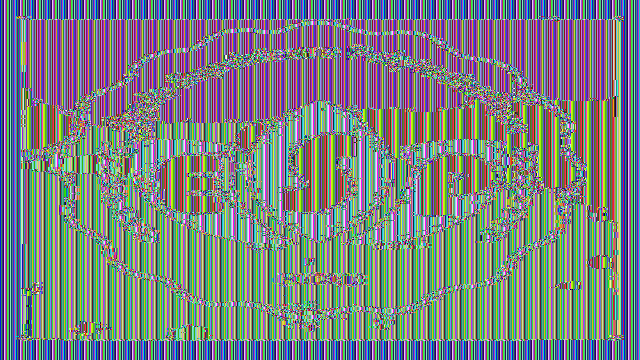
\includegraphics[width=\linewidth]{img/esp_plat_ecb.png}\\[0.2em]
      \small\textbf{\textcolor{espred}{AES-ECB}}
    \column{0.32\textwidth}\centering
      
\includegraphics[width=\linewidth]{img/esp_plat_cbc.png}\\[0.2em]
      \small\textbf{\textcolor{espgreen}{AES-CBC}}
  \end{columns}
  \vspace{0.6em}
  \begin{itemize}\small
    \item \textbf{Même AES, même clé} : seul le mode change. En ECB, \alert{le sceau et « ESP » restent lisibles} (comme le célèbre manchot).
    \item \textbf{ECB fuit d'autant plus que les données se répètent} : logo plat \textbf{98,6\,\%} de blocs répétés $\Rightarrow$ très visible ;
          photo du logo \textbf{23\,\%} $\Rightarrow$ à peine visible. Les données de paiement : \textbf{75\,\%} (E2).
    \item CBC : chaque bloc dépend du précédent et de l'IV $\Rightarrow$ 0\,\% de répétition, du bruit.
  \end{itemize}
\end{frame}

\begin{frame}{Expérimentation : tous les cas de figure, mesurés}
  \begin{columns}[T]
    \column{0.50\textwidth}
    \scriptsize\textbf{E1 --- Jeu IND-CPA programmé} (2\,000 parties par configuration)\\[0.2em]
    \begin{tabular}{lcc}
      \toprule
      Configuration & Avantage & Verdict \\
      \midrule
      ECB & 1,000 & \textcolor{espred}{cassé} \\
      CBC, IV fixe & 1,000 & \textcolor{espred}{cassé} \\
      CBC, IV prévisible & 1,000 & \textcolor{espred}{cassé} \\
      CBC, IV aléatoire & 0,039 & \textcolor{espgreen}{sûr} \\
      CTR, nonce fixe & 1,000 & \textcolor{espred}{cassé} \\
      CTR, nonce aléatoire & 0,021 & \textcolor{espgreen}{sûr} \\
      GCM, nonce fixe & 1,000 & \textcolor{espred}{cassé} \\
      GCM, nonce aléatoire & 0,009 & \textcolor{espgreen}{sûr} \\
      \bottomrule
    \end{tabular}\\[0.2em]
    \tiny Avantage $= |2\Pr[\text{gagner}] - 1|$ : 0 = l'attaquant devine au hasard, 1 = il gagne à tous les coups.
    \column{0.48\textwidth}
    \scriptsize
    \begin{itemize}
      \item \textbf{E2 --- Fuite ECB} : sur un journal de 2\,000 transactions, \alert{75\,\%} des blocs chiffrés
            se répètent en ECB (autant que dans le clair) ; \textbf{0\,\%} en CBC, CTR, GCM.
      \item \textbf{E3 --- Un bit modifié} : ECB, CBC et CTR acceptent le message ; en CTR la modification est
            \alert{contrôlée bit pour bit}. \textbf{Seul GCM la rejette.}
      \item \textbf{E4 --- Oracle de remplissage} \cite{vaudenay2002} : message CBC de 3 blocs
            \alert{déchiffré sans la clé} en 5\,760 requêtes (0,04\,s).
      \item \textbf{E5 --- Nonce réutilisé} : le second message est lu sans la clé, \alert{en CTR comme en GCM}.
    \end{itemize}
    \vspace{0.2em}
    \tiny Banc d'essai reproductible : \texttt{demo/banc\_essai.py} (Python 3, \texttt{cryptography} 50.0), données synthétiques, graine fixe (résultats identiques à chaque exécution), moins de 5\,s au total.
  \end{columns}
\end{frame}

% =====================================================================
\section{État de l'art}

\begin{frame}{État de l'art et positionnement}
  \centering\scriptsize
  \begin{tabular}{p{2.7cm}p{5.4cm}p{4.4cm}}
    \toprule
    \textbf{Référence} & \textbf{Apport} & \textbf{Limite} \\
    \midrule
    \textbf{Egele et al.}, CCS 2013 \cite{egele2013} &
      Applis Android : \textbf{10\,327 sur 11\,748} applis utilisant des API de chiffrement (\textbf{88\,\%}) font au moins une erreur. &
      Ni centré paiement ni Afrique de l'Ouest : les 88\,\% \textbf{ne se transposent pas}. \\
    \textbf{Rahaman et al.}, CCS 2019 \cite{rahaman2019} (CryptoGuard) &
      46 projets Apache, 6\,181 applis Android ; fausses alertes réduites de 76 à 80\,\% ; \textbf{98,6\,\%} de précision sur 1\,295 alertes Apache vérifiées. &
      Précision mesurée sur Apache, pas sur des applis de paiement. \\
    \textbf{Diallo et al.}, 2024 \cite{diallo2024} &
      \textbf{59 applis bancaires de l'UEMOA} : modes de chiffrement non sûrs \textbf{32\,\%},
      clés en dur \textbf{20\,\%}. &
      \textbf{Exclut le mobile money}. \\
    \textbf{Reaves et al.}, ACM TOPS 2017 \cite{reaves2017} &
      Étude de \textbf{46 applications de mobile money}. & Pas centrée sur les modes AES. \\
    Muslukhov et al., 2018 \cite{muslukhov2018} & Les erreurs viennent surtout des \textbf{bibliothèques tierces}. & Pas centré sur le paiement. \\
    \bottomrule
  \end{tabular}\\[0.3em]
  \raggedright\scriptsize
  \textbf{Ce qui manque}, à notre connaissance : une étude des \textbf{applis de paiement ouest-africaines, mobile money compris},
  centrée sur les \textbf{modes AES}, avec une \textbf{mesure des faux positifs}.\\[0.2em]
  \textbf{Notre contribution} : mesurer cet écart à la règle d'or (AES-GCM, nonce unique, clé hors du code),
  de façon \textbf{reproductible et éthique}, et comparer avec 2013, 2019 et les applis bancaires de l'UEMOA.
\end{frame}

% =====================================================================
\section{Conclusion}

\begin{frame}{À retenir}
  \begin{block}{Trois messages}
    \begin{enumerate}
      \item \textbf{AES n'est pas cassé : ce sont les usages} (mode, IV, nonce, clé). Même GCM tombe si le nonce est réutilisé.
            Règle d'or : \textbf{AES-GCM, nonce unique, clé hors du code}.
      \item Les erreurs sont fréquentes à grande échelle (\textbf{88\,\%} chez Egele et al.), mais une alerte statique
            reste \textbf{un indice à vérifier} : faux positifs et faux négatifs, comme notre pilote l'a montré.
      \item Notre projet mesure, de façon \textbf{reproductible et éthique}, la fréquence de ces erreurs dans un corpus documenté
            d'APK de paiement Android utilisées en Afrique de l'Ouest.
    \end{enumerate}
  \end{block}
\end{frame}

\begin{frame}{Questions de quiz}
  \scriptsize
  \begin{columns}[T]
    \column{0.32\textwidth}
    \textbf{1. Quel mode laisse voir les motifs d'une image ?}\\
    a) CBC \quad b) \textbf{ECB} \quad c) CTR \quad d) GCM
    \column{0.32\textwidth}
    \textbf{2. En CTR, réutiliser le nonce permet à Kiné de calculer\ldots}\\
    a) la clé \quad b) \textbf{$m \oplus m'$} \quad c) le haché \quad d) rien
    \column{0.32\textwidth}
    \textbf{3. Quel mode assure confidentialité \emph{et} intégrité ?}\\
    a) ECB \quad b) CBC \quad c) CTR \quad d) \textbf{GCM}
  \end{columns}
\end{frame}

\begin{frame}{Références}
  \setbeamertemplate{bibliography item}[text]
  \setbeamerfont{bibliography item}{size=\tiny}
  \setbeamerfont{bibliography entry author}{size=\tiny}
  \setbeamerfont{bibliography entry title}{size=\tiny}
  \setbeamerfont{bibliography entry location}{size=\tiny}
  \setbeamerfont{bibliography entry note}{size=\tiny}
  \tiny
  \begin{multicols}{2}
  \begin{thebibliography}{99}\setlength{\itemsep}{2pt}\renewcommand{\newblock}{\ }
    \bibitem{egele2013} M.~Egele, D.~Brumley, Y.~Fratantonio, C.~Kruegel.
      \newblock An Empirical Study of Cryptographic Misuse in Android Applications.
      \newblock \emph{ACM CCS}, 2013, p.~73--84. DOI 10.1145/2508859.2516693.
    \bibitem{rahaman2019} S.~Rahaman, Y.~Xiao, S.~Afrose \emph{et al.}
      \newblock CryptoGuard: High Precision Detection of Cryptographic Vulnerabilities in Massive-sized Java Projects.
      \newblock \emph{ACM CCS}, 2019, p.~2455--2472. DOI 10.1145/3319535.3345659.
    \bibitem{nist38a} M.~Dworkin.
      \newblock \emph{SP 800-38A : Recommendation for Block Cipher Modes of Operation}. NIST, 2001.
    \bibitem{nist38d} M.~Dworkin.
      \newblock \emph{SP 800-38D : Galois/Counter Mode (GCM) and GMAC}. NIST, 2007.
    \bibitem{fips197} NIST.
      \newblock \emph{FIPS 197 : Advanced Encryption Standard (AES)}. 2001, mise à jour 2023.
    \bibitem{vaudenay2002} S.~Vaudenay.
      \newblock Security Flaws Induced by CBC Padding -- Applications to SSL, IPSEC, WTLS\ldots
      \newblock \emph{EUROCRYPT 2002}, LNCS 2332, p.~534--545.
    \bibitem{joux2006} A.~Joux.
      \newblock Authentication Failures in NIST Version of GCM.
      \newblock Commentaire public adressé au NIST, 2006.
    \bibitem{bceao2024} BCEAO.
      \newblock \emph{Rapport annuel sur l'évolution des services financiers numériques dans l'UEMOA au titre de l'année 2024}.
      \newblock Janvier 2026, \S\,11 (p.~14) et \S\,19 (p.~17).
    \bibitem{cbumoa2025} Commission bancaire de l'UMOA.
      \newblock \emph{Rapport annuel 2025}. 2026, p.~141 et annexe des EME p.~340 (PDF).
    \bibitem{muslukhov2018} I.~Muslukhov, Y.~Boshmaf, K.~Beznosov.
      \newblock Source Attribution of Cryptographic API Misuse in Android Applications.
      \newblock \emph{ACM AsiaCCS}, 2018.
    \bibitem{diallo2024} A.~Diallo, A.~War, M.~A.~Diouf, J.~Samhi, S.~Arzt, T.~F.~Bissyandé, J.~Klein.
      \newblock Security Assessment of Mobile Banking Apps in West African Economic and Monetary Union.
      \newblock arXiv:2411.04068, 2024.
    \bibitem{reaves2017} B.~Reaves, J.~Bowers, N.~Scaife, A.~Bates, A.~Bhartiya, P.~Traynor, K.~R.~B.~Butler.
      \newblock Mo(bile) Money, Mo(bile) Problems: Analysis of Branchless Banking Applications.
      \newblock \emph{ACM Transactions on Privacy and Security}, 20(3), art.~11, 2017. DOI 10.1145/3092368.
    \bibitem{paar2024} C.~Paar, J.~Pelzl, T.~Güneysu.
      \newblock \emph{Understanding Cryptography}, 2\textsuperscript{e} éd. Springer, 2024.
  \end{thebibliography}
  \end{multicols}
\end{frame}

% =====================================================================
%  Annexes : conservées dans le source, mais exclues du PDF de remise
%  pour respecter la limite de 12 diapositives du chapitre 00.
% =====================================================================
\iffalse
\appendix

\begin{frame}[fragile]{Annexe A --- Ce que voit le destinataire après une attaque}
  \scriptsize
\begin{verbatim}
CTR, nonce réutilisé : Kiné connaît m1 et calcule c2 xor (c1 xor m1)
   m2 retrouvé SANS la clé : VIRE 7500 FCFA A AWA    ; PIN=4821

CTR sans intégrité : Modou applique delta = '5' xor '9' au chiffré
   message envoyé      : VIRE 5000 FCFA A MOUSSA
   la banque déchiffre : VIRE 9000 FCFA A MOUSSA   <- personne ne s'en rend compte

AES-GCM, même modification
   la banque vérifie le tag : InvalidTag -> message REJETÉ
\end{verbatim}
  \centering
  \begin{tabular}{lcccc}
    \toprule
    Un bit modifié dans le bloc 2 & ECB & CBC & CTR & GCM \\
    \midrule
    Message accepté ? & oui & oui & oui & \textcolor{espgreen}{\textbf{non}} \\
    Octets du clair modifiés & 16 & 17 & 1 & -- \\
    Blocs touchés & 2 & 2 et 3 & 2 & -- \\
    Modification contrôlable ? & non & oui (bloc 3) & \textcolor{espred}{oui, bit à bit} & rejetée \\
    \bottomrule
  \end{tabular}
\end{frame}

\begin{frame}{Annexe B --- Débit : la sécurité ne coûte rien}
  \centering
  \begin{tabular}{lrr}
    \toprule
    Algorithme & Débit (Mo/s), min -- max & GCM / CBC \\
    \midrule
    AES-128-ECB & 457 -- 1\,402 & \\
    AES-128-CBC & 429 -- 904 & \\
    AES-128-CTR & 985 -- 2\,096 & \\
    \textbf{AES-128-GCM} & \textbf{944 -- 1\,861} & \textbf{2,1 à 2,3} \\
    ChaCha20-Poly1305 & 600 -- 1\,234 & \\
    \bottomrule
  \end{tabular}\\[0.6em]
  \small 3 lancements complets (64 Mo, médiane de 5 mesures), Intel Core i5-1335U (AES-NI), \texttt{cryptography} 50.0.\\
  Les débits absolus \textbf{varient du simple au double} selon l'état de la machine (alimentation, charge),
  mais \textbf{GCM reste environ 2 fois plus rapide que CBC à chaque lancement} : aucune excuse pour un mauvais mode.\\
  \scriptsize CBC est séquentiel (chaque bloc attend le précédent) ; CTR et GCM se parallélisent.
  ChaCha20 brille sur les téléphones sans AES matériel.
\end{frame}


\begin{frame}{Annexe C --- Schémas ECB et CBC sur l'ordre de virement}
  \small Message de 3 blocs de 16 octets, dont \textbf{deux identiques} :
  \texttt{DEST:MOUSSA\_\_\_\_\_} \;|\; \texttt{MONTANT:5000FCFA} \;|\; \texttt{MONTANT:5000FCFA}
  \vspace{0.3em}

  \begin{columns}[T]
    \column{0.48\textwidth}
    \centering\textbf{ECB} : $c_i = E_K(m_i)$\\[0.3em]
    \begin{tikzpicture}
      \foreach \i/\x in {1/0,2/1.7,3/3.4}{
        \node[blk] (m\i) at (\x,0) {$m_\i$};
        \node[aes] (e\i) at (\x,-0.9) {$E_K$};
        \draw[arr] (m\i) -- (e\i);
      }
      \node[blk, fill=espblue!25] (c1) at (0,-1.8) {\texttt{9f3a\ldots}};
      \node[blk, fill=espred!25] (c2) at (1.7,-1.8) {\texttt{41c7\ldots}};
      \node[blk, fill=espred!25] (c3) at (3.4,-1.8) {\texttt{41c7\ldots}};
      \foreach \i in {1,2,3}{\draw[arr] (e\i) -- (c\i);}
    \end{tikzpicture}\\[0.2em]
    \footnotesize\textcolor{espred}{$c_2 = c_3$ : Kiné voit que les blocs se répètent.}

    \column{0.48\textwidth}
    \centering\textbf{CBC} : $c_i = E_K(m_i \oplus c_{i-1})$, $c_0 = \mathit{IV}$\\[0.3em]
    \begin{tikzpicture}
      \node[blk, minimum width=0.8cm] (iv) at (-1.2,-0.45) {IV};
      \foreach \i/\x in {1/0,2/1.7,3/3.4}{
        \node[blk] (m\i) at (\x,0) {$m_\i$};
        \node[xorn] (x\i) at (\x,-0.45) {};
        \draw (x\i.north)--(x\i.south) (x\i.west)--(x\i.east);
        \node[aes] (e\i) at (\x,-1.05) {$E_K$};
        \draw[arr] (m\i) -- (x\i); \draw[arr] (x\i) -- (e\i);
      }
      \node[blk, fill=espblue!25] (c1) at (0,-1.85) {\texttt{9f3a\ldots}};
      \node[blk, fill=espgreen!25] (c2) at (1.7,-1.85) {\texttt{d012\ldots}};
      \node[blk, fill=espblue!15] (c3) at (3.4,-1.85) {\texttt{7be8\ldots}};
      \foreach \i in {1,2,3}{\draw[arr] (e\i) -- (c\i);}
      \draw[arr] (iv) -- (x1);
      \draw[arr] (c1.east) -| ($(x2.west)+(-0.35,0)$) -- (x2.west);
      \draw[arr] (c2.east) -| ($(x3.west)+(-0.35,0)$) -- (x3.west);
    \end{tikzpicture}\\[0.2em]
    \footnotesize\textcolor{espgreen}{Blocs égaux $\Rightarrow$ chiffrés différents.}
  \end{columns}
  \vspace{0.2em}
  \centering\scriptsize Valeurs hexadécimales illustratives.
\end{frame}

\begin{frame}{Annexe D --- Pilote de l'analyse statique (12 APK F-Droid)}
  \begin{columns}[T]
    \column{0.50\textwidth}
    \scriptsize
    \textbf{Corpus reproductible}
    \begin{itemize}
      \item Catalogue public F-Droid, catégories finance et portefeuilles : \textbf{70 éligibles}, \textbf{12 tirées au hasard} (graine fixe).
      \item \textbf{12/12 empreintes SHA-256} vérifiées contre celles de F-Droid.
      \item 2 applis Flutter \textbf{non analysables} (code natif) : comptées à part.
    \end{itemize}
    \textbf{Outil validé avant de mesurer}
    \begin{itemize}
      \item v1 : un \alert{faux positif} trouvé par vérification manuelle $\Rightarrow$ suivi de provenance.
      \item v2 : des \alert{faux négatifs} révélés par un \textbf{témoin vulnérable} (appli bancaire d'entraînement, volontairement vulnérable) $\Rightarrow$ analyse inter-procédurale.
      \item v3 : témoin \textbf{3/3} (clé en dur, IV à zéros, CBC sans MAC).
    \end{itemize}
    \column{0.47\textwidth}
    \scriptsize
    \begin{tabular}{lr}
      \toprule
      Applis analysables & 10 \\
      Utilisent l'API de chiffrement & 5 \\
      Avec $\geq 1$ erreur & \textbf{0 / 5} \\
      Prévalence (IC 95\,\% de Wilson) & 0\,\% [0 ; 43\,\%] \\
      \bottomrule
    \end{tabular}\\[0.4em]
    \textbf{Lecture honnête} : 5 applis ne suffisent pas pour conclure (l'intervalle va jusqu'à 43\,\%),
    et des applis open source de budget ne représentent pas le mobile money de l'UEMOA.
    Le pilote prouve que \textbf{la chaîne fonctionne} ; le corpus complet vise Google Play (UEMOA).
  \end{columns}
\end{frame}

\fi
\end{document}
